\section{Results}
\label{sec:results}

\subsection{Genotypes}
\label{sec:genotypes}  
GBS detected 32\,706, 40\,734 and 166\,418 SNP loci in Alfalfa-PV, Alfalfa-Med and Rice, respectively (Table~\ref{tab:descriptive_statistics}). The overall missing rate was $66.6\%$, $59.6\%$ and $53.4\%$ in the three datasets. Supplementary Figure S1 shows the density distribution of missing rate per markers in the complete datasets. The amount of missing marker genotypes varied with the threshold of maximum per-marker missing-rate allowed in the data (10\%, 20\%, 40\% and 70\%) and the proportion of artificial missing genotypes that were introduced (1\%, 5\%, 10\% and 20\%). Missing data point counts ranged from a minimum of 3\,878 in Alfalfa-PV with 10\% allowed and 1\% artificial missing genotypes, to a maximum of 5\,580\,616 in Rice with 70\% allowed and 20\% artificial missing genotypes. Over all datasets and allowed/artificial missing genotypes thresholds, the amount of missing data points to be imputed averaged 249\,405.\\
Minor Allele Frequency (MAF) was 0.172, 0.170 and 0.140 in Alfalfa-PV, Alfalfa-Med and Rice, respectively. The three datasets were therefore unbalanced with respect to genotype classes: Rice had the lowest MAF, while Alfalfa-PV and Alfalfa-Med had the smallest minor classes (minor homozygotes 3.5\% and 3.2\% of the total genotypes). Figure~\ref{fig:genotype_classes} reports the proportion of genotypes in each class in the complete datasets (100\%) and as a function of the maximum allowed missing rate per marker. The relative proportion of genotype classes remained approximately stable in rice. In contrast, the heterozygous class in alfalfa tended to become smaller with increasing proportion of allowed genotypes. This reflected the different GBS calling criteria for homozygous and heterozygous SNP: heterozygous SNPs required fewer overlapping reads to be called, while the implemented quality filters on alfalfa required a larger number of reads to call a homozygous loci. The average missing-rate and MAF in the 12 rice chromosomes were comparable to the whole-rice dataset.

\begin{figure}
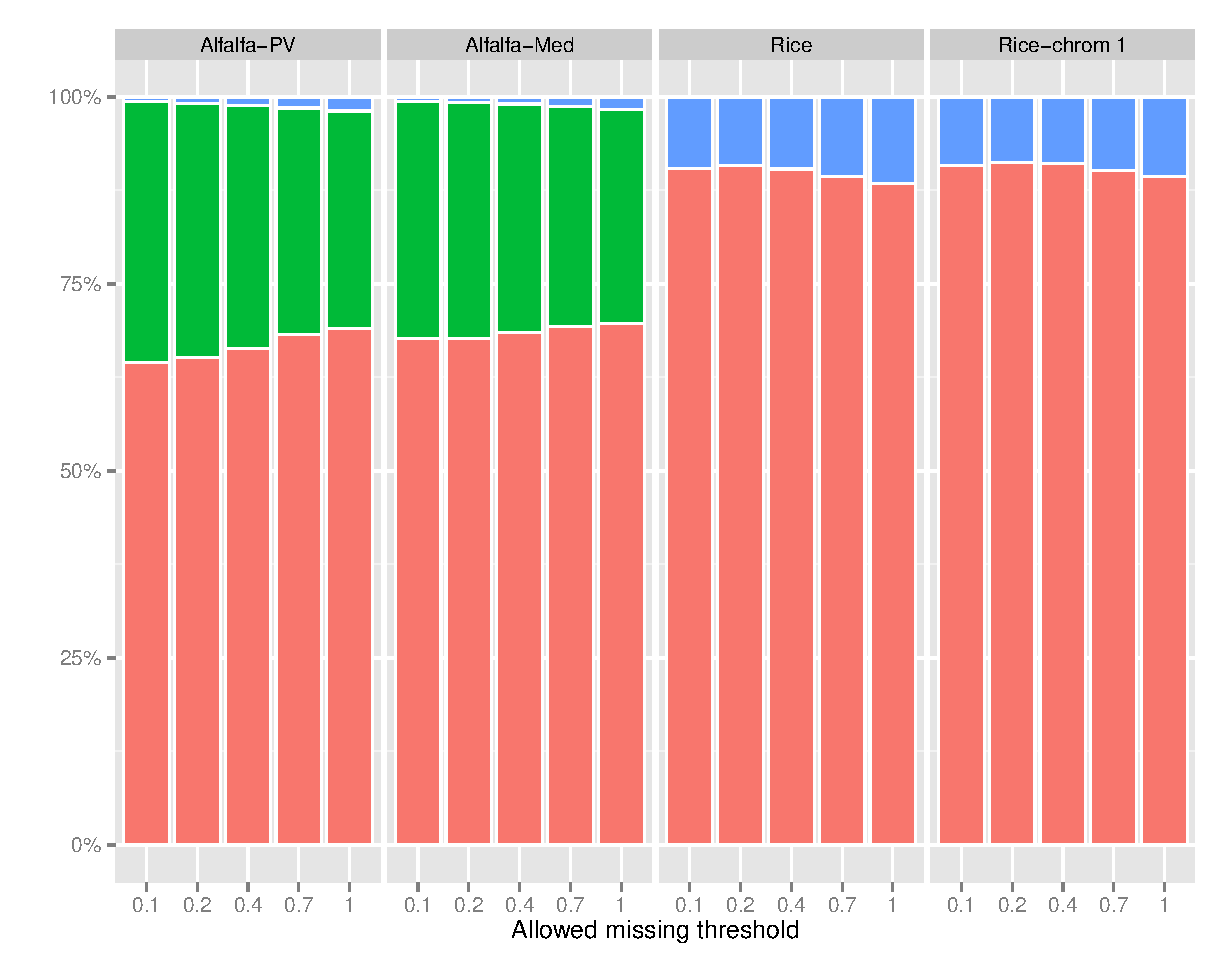
\includegraphics[width=0.95\textwidth]{Fig01_class_breakdown_all.pdf}
\caption[Proportions of genotype classes]{​Proportion of genotype classes for the different missing rate thresholds (0.1, 0.2, 0.4, 0.7 and 1 -the complete dataset), in Alfalfa-PV, Alfalfa-Med and Rice (all chromosomes and chromosome 1 only). Red bars represents the most common homozygous (AA), blue bars the least common homozygous (BB) and green bars the heterozygous (AB).}
\label{fig:genotype_classes}
\end{figure}

\subsection{Imputation accuracy}
\label{sec:imputation_accuracy}  

In rice, the average imputation accuracy over all genotypic classes was close to 100\% with most methods and still above 90\% at maximum proportions of allowed (70\%) and artificial (20\%) missing genotypes (Figure~\ref{fig:accuracy_rice}). The overall accuracy for alfalfa, averaged across the two datasets, was 12-25\% lower than rice, ranging between 66\% and 84\% (Figure~\ref{fig:accuracy_alfalfa}). The imputation accuracy varied across the different genotype classes, with the highest accuracy in the most common genotype class (averaging 90.8\% and 99.3\% in alfalfa and rice, respectively), while the least common genotype class showed much lower accuracy (averaging 4.1\% and 73.4\% in alfalfa and rice, respectively). Alfalfa datasets included heterozygous SNP loci, accounting for an average of 30\% of individuals per locus (Table~\ref{tab:descriptive_statistics}). Heterozygotes had an intermediate imputation accuracy ranging from 0\% with MNI to 70\% with KNNI. Results for each individual alfalfa population, the 12 individual rice chromosomes, and the whole rice dataset are similar to those discussed here (see Supplementary Figures S2 to S16). \\
Missing data did not affect the imputation accuracy substantially, with most algorithms showing a flat or almost flat response to increased missing rate. KNNI showed a decreasing imputation accuracy with increasing missing data, both in alfalfa and rice.\\
In rice, Beagle outperformed all other imputation methods, making efficient use of marker position (Figure~\ref{fig:accuracy_rice}). When markers were randomly reshuffled (thus offsetting position information), though, general imputation methods (other than MNI) showed a higher imputation accuracy than Beagle. In general we observed for all thresholds and in both genotype classes the following ranking of methods for imputation accuracy: RFI $>$ KNNI $>$ SVDI.
In particular, for 70\% allowed missing rate datasets, the imputation accuracy of RFI was still greater than 90\%, while it dropped towards 75\% for KNNI and SVDI. As expected, MNI had an imputation accuracy of 100\% in the major homozygous class, but dropped to 0\% in the minor homozygous class.\\
In alfalfa KNNI showed the highest imputation accuracy over all classes and in the heterozygous and minor homozygous genotype classes (Figure~\ref{fig:accuracy_alfalfa}). RFI and SVDI were second ranking. They did not differ much from MNI in the overall accuracy and in the major homozygous class, but gave higher imputation accuracy in the heterozygous and minor homozygous classes. Beagle was also applied to alfalfa, where the relative position of markers in the genome is not known. The overall imputation accuracy with Beagle was about 67\%, with accuracies of almost 100\% in the major homozygous class but practically 0\% in the heterozygous and minor homozygous classes.

\begin{figure}
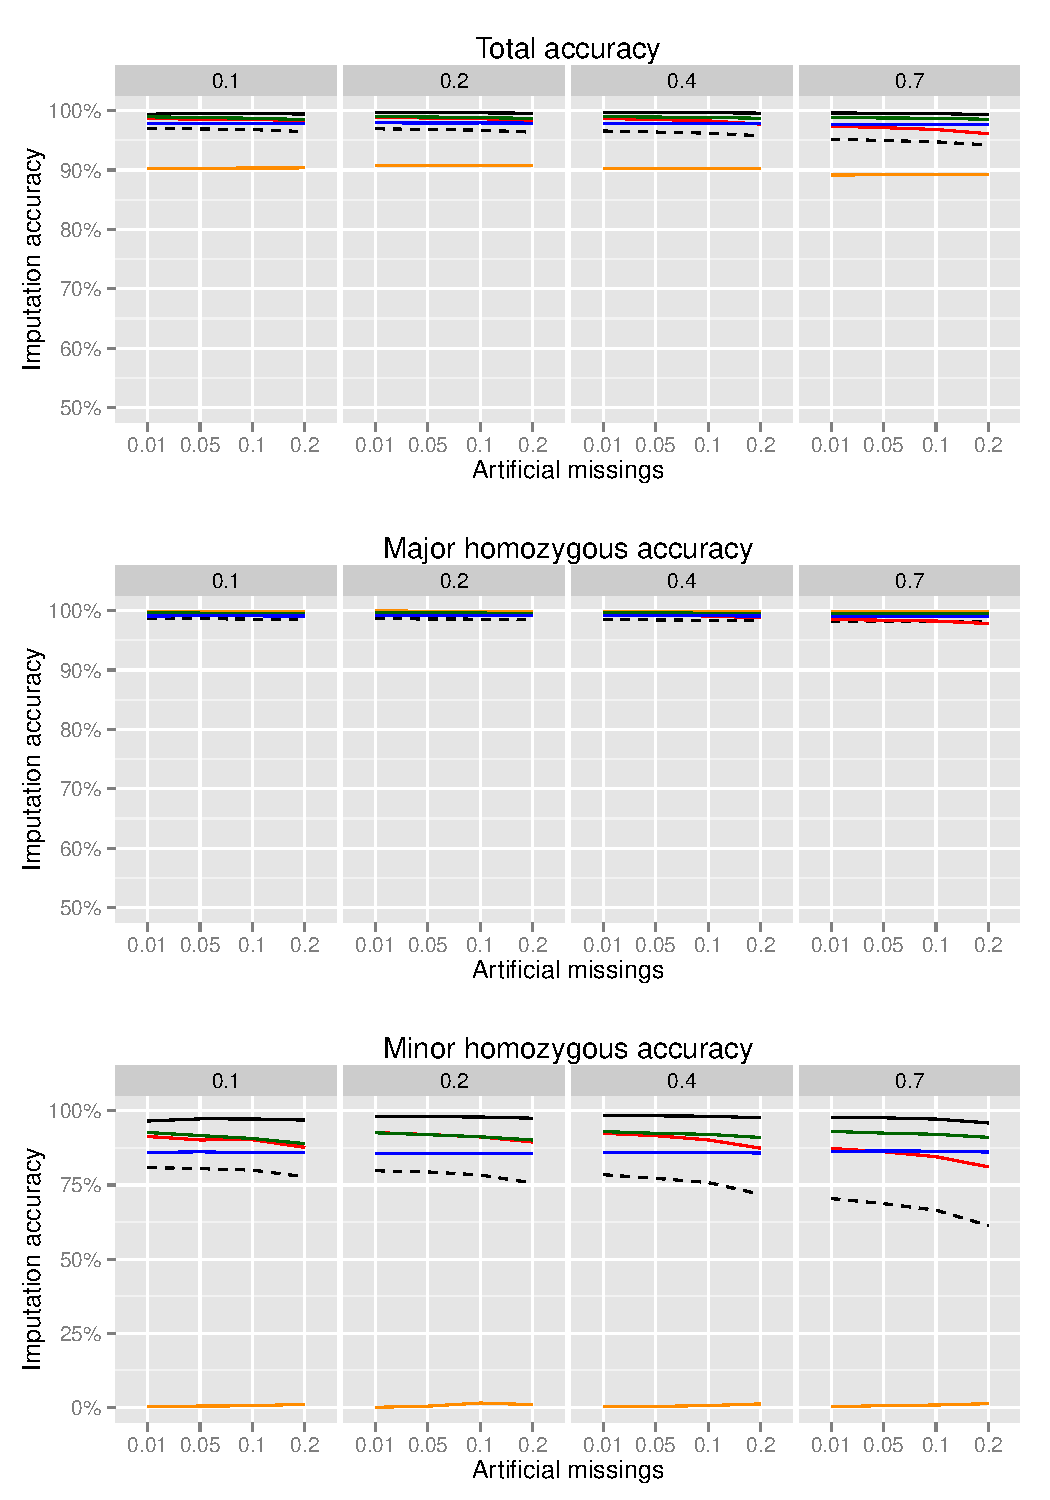
\includegraphics[width=0.95\textwidth]{Fig02_Rice-chrom_avg.pdf}
\caption[Rice imputation accuracies]{
imputation accuracies overall, for the major homozygous genotype (AA), and for the minor homozygous genotype (BB) in datasets consisting of 10\%, 20\%, 40\% and 70\% allowed missing data per locus (boxes) with 1\%, 5\%, 10\% and 20\% additional missing values artificially introduced (x-axis) averaged over the 12 rice chromosomes. Lines colors represent the five imputation algorithms: MNI (orange), KNNI (red), SVDI (blue), RFI (green), Beagle with ordered markers (solid black) and Beagle with unordered markers (dashed black).}
\label{fig:accuracy_rice}
\end{figure}

\begin{figure}
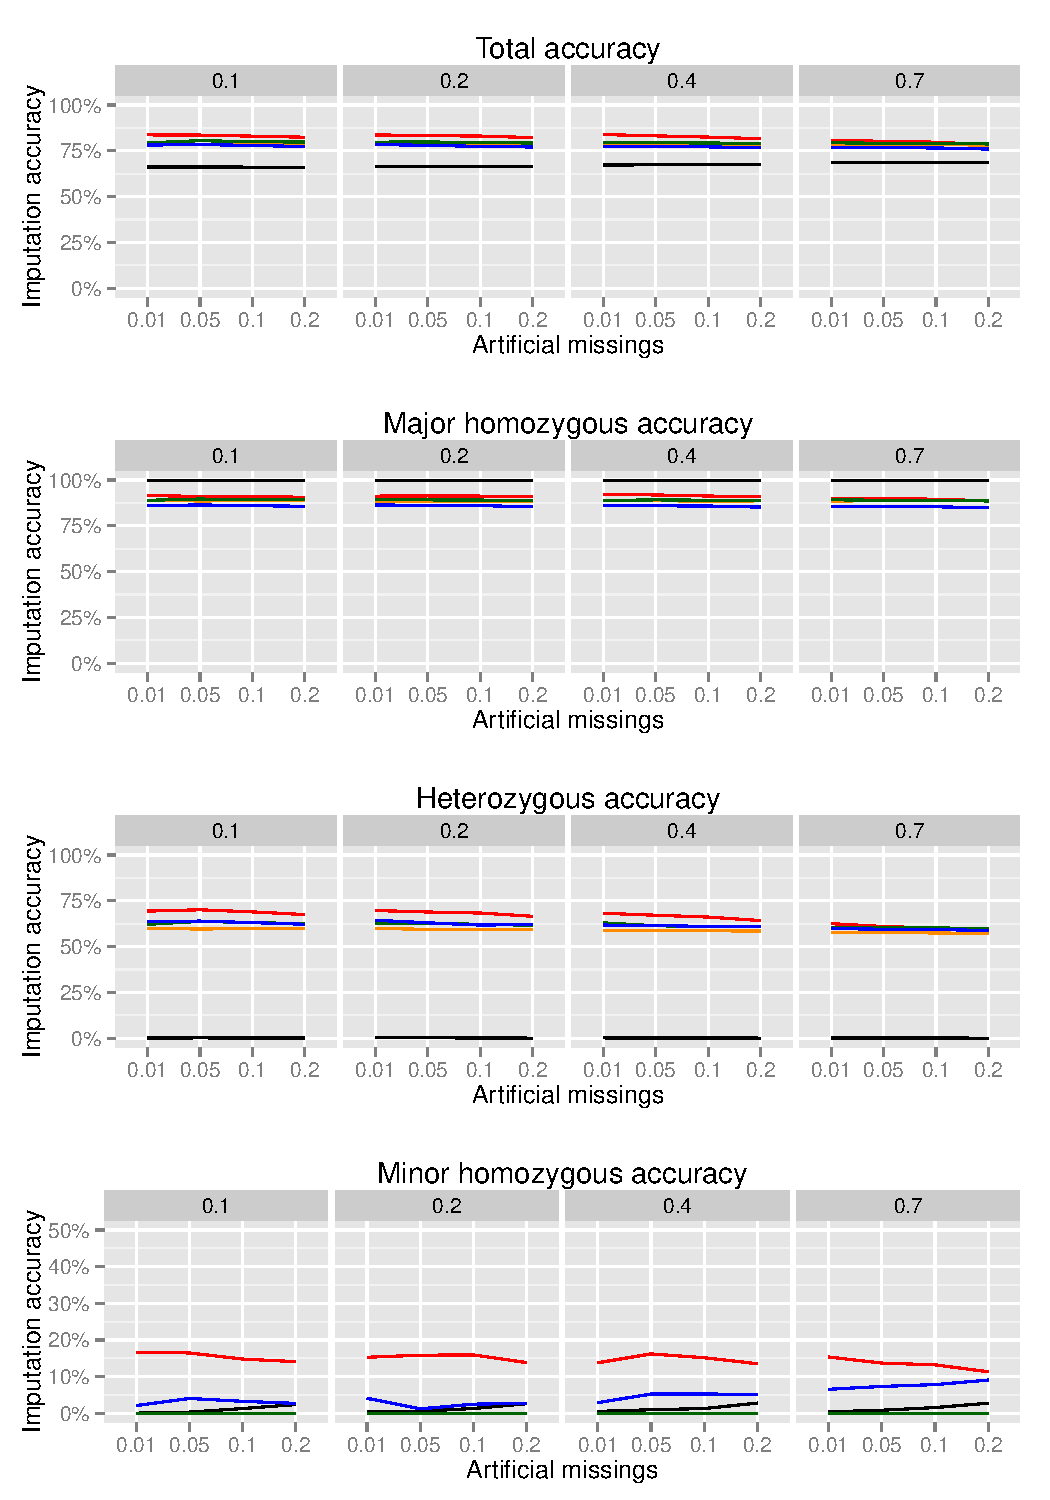
\includegraphics[width=0.95\textwidth]{Fig03_Alfalfa_avg.pdf}
\caption[Alfalfa imputation accuracies]{
imputation accuracies overall, for the major homozygous genotype (AA), for heterozygotes (AB), and for the minor homozygous genotype (BB) in datasets consisting of 10\%, 20\%, 40\% and 70\% allowed missing data per locus (boxes) with 1\%, 5\%, 10\% and 20\% additional missing values artificially introduced (x-axis) averaged two alfalfa populations (Alfalfa-Med and Alfalfa-PV). Lines colors represent the five imputation algorithms: MNI (orange), KNNI (red), SVDI (blue), RFI (green) and Beagle (black).}
\label{fig:accuracy_alfalfa}
\end{figure}

\subsection{Computation time}
\label{sec:computation_time}  
The amount of time required to complete the imputation process was recorded for each method. Only the implementation of RFI could leverage a multi-core/multi-thread environment, so that RFI computation times should be evaluated considering 10 CPUs used in parallel, while all other algorithms used only one CPU at a time.\\
Imputation efficiency (Figure~\ref{fig:time_analysis}) was assessed with respect to the gross dimension of the data set (i.e., number of markers $\times$ number of samples) and to the total number of missing genotypes to be imputed (e.g., 341\,097 missing genotypes for the Alfalfa-Med population with 40\% missing rate and 20\% artificial missing).
RFI required by far the longest computation times (in spite of 10-core/thread parallelization), which grew approximately exponentially ($O(e^N)$) with problem size, and easily required tens of hours for individual rice chromosomes, and hundred of hours (up to 937 hours) for the complete rice dataset. The second slowest algorithm was KNNI, with computation times growing approximately quadratically ($O(N^2)$) with problem complexity (the chosen KNNI implementation contains no heuristic method to prune the all vs. all distance calculation). KNNI was however significantly faster than RFI (on average 16.7 times faster), requiring a time ranging from 20.68 seconds (rice chromosome 7, 10\% allowed, 1\% artificial) to about 28 hours (rice complete dataset, 70\% allowed, 20\% artificial) to complete the imputation task.\\
All other algorithms were faster, with computation times growing linearly or logarithmically with problem size. Beagle and SVDI resulted in similar execution times. MNI was by far the fastest imputation algorithm, being scarcely affected by the size of the problem (computation times ranging from 0.23 to 31.29 seconds).

\begin{figure}
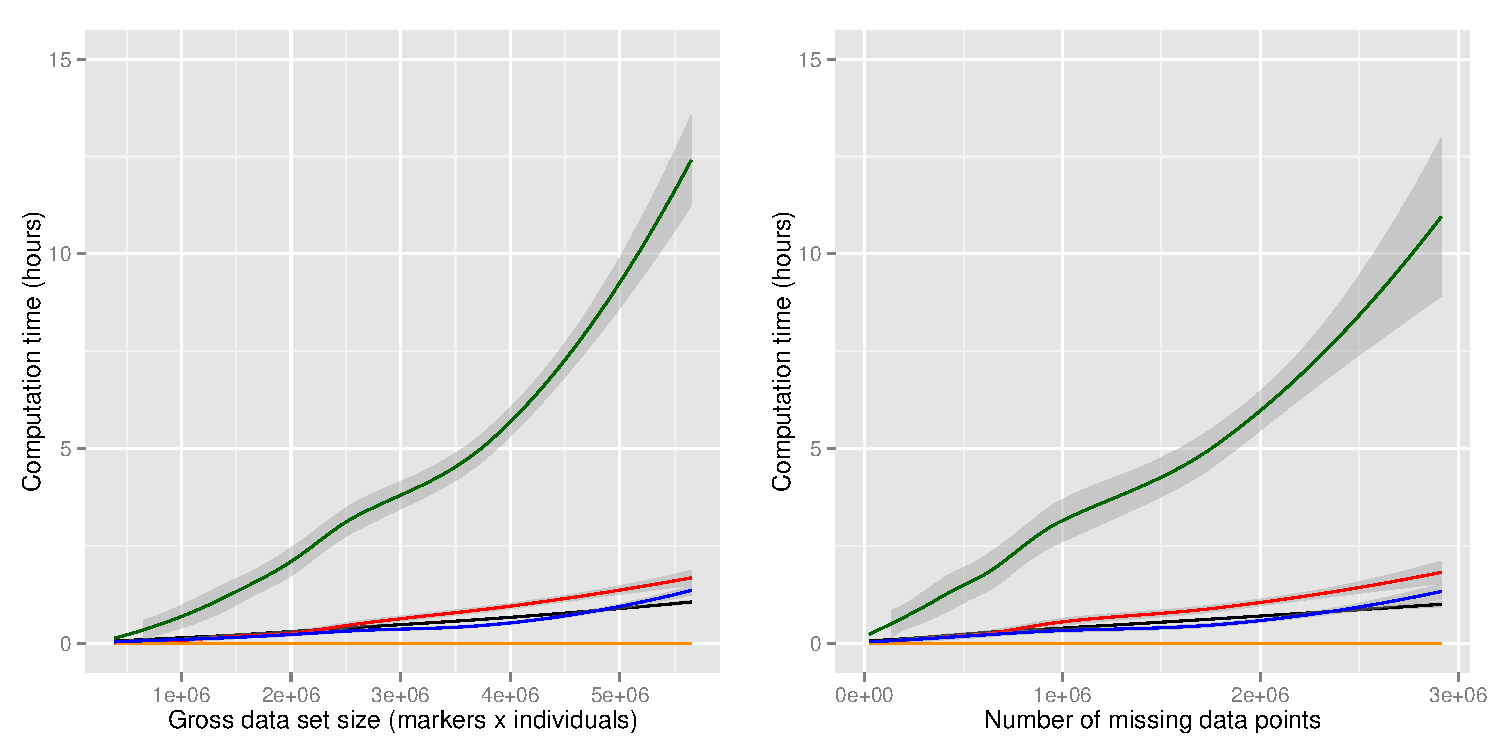
\includegraphics[width=0.95\textwidth]{Fig04_time_analysis.pdf}
\caption[Computation times]{computation time as a function of the amount of the total size of the imputed dataset (left) and of missing data (right) for the five imputation methods (MNI: orange, KNNI: red, SVDI: blue, RFI: green, Beagle:black). Plots include measures on Alfalfa-Med population, Alfalfa-PV population, and rice chromosomes 1 to 12. Complete rice datasets are omitted for readibility.}
\label{fig:time_analysis}
\end{figure}
